% -----------------------------------------------
% Template for ISMIR Papers
% 2018 version, based on previous ISMIR templates

% Requirements :
% * 6+n page length maximum
% * 4MB maximum file size
% * Copyright note must appear in the bottom left corner of first page
% * Clearer statement about citing own work in anonymized submission
% (see conference website for additional details)
% -----------------------------------------------

\documentclass{article}
\usepackage{ismir,amsmath,cite,url}
\usepackage{graphicx}
\usepackage{color}


% Title.
% ------
\title{GraphDitty: A Software Suite for Geometric Music Structure Visualization}

% Note: Please do NOT use \thanks or a \footnote in any of the author markup

% Single address
% To use with only one author or several with the same address
% ---------------
\oneauthor
 {Christopher J. Tralie}
 {Duke University Department of Mathematics}



\sloppy % please retain sloppy command for improved formatting
\graphicspath{{Figures/}}

\begin{document}

%
\maketitle
%
\begin{abstract}
    In this work, we present a new twist on music structure analysis and visualization.  We devise a technique\footnote{This is a refinement of / followup to our prior works ``scaffolding and spines'' \cite{bendichgeometric} and ``Loop Ditty'' \cite{tralie2017Dissertation}} to create clean audio self-similarity matrices at the song level by fusing multiple features upstream.  We then derive multiple geometric features from this representation to elucidate hierarchical structure, including Laplacian eigenvectors, spring graph layouts, and diffusion maps.  We then provide a suite of Javascript visualization tools to view the SSMs and derived features synchronized with the audio they represent.  Our code is clean with the help of Numpy/Scipy/Librosa on the Python end and d3.js on the Javascript end, but it can be treated as a blackbox for users who would like to engage with the visualizations without delving into the technical details.  Code can be found at \url{http://www.github.com/ctralie/GraphDitty}, and a live demo is present at \url{http://www.covers1000.net/GraphDitty}.
\end{abstract}


\section{Similarity fusion}\label{sec:fusion}

The self-similarity matrix (SSM) is a common data structure through which to visualize recurrence in musical audio.  For a particular feature type, the SSM is a symmetric distance matrix $D$ which records all pairwise distances between windows in time, as measured by that feature.  Let $D^C$ be a matrix measuring the cosine distance between stacked-delayed\footnote{We use stack-delayed features to promote diagonal structures, as shown in \cite{tralie2017quasi}}\cite{serra2009cross} chroma features, and let $D^M$ be a matrix measuring the Euclidean distance between stack-delayed MFCCs.  The we can apply a {\em similarity kernel} to each of them so that $W^C_{ij} = \exp (-(D^C_{ij})^2 / (2 \sigma_{ij}^2) )$, and likewise for $W^M$ for $D^M$, where $\sigma_{ij}$ is a mutual nearest neighbor autotuned distance (see \cite{wang2012unsupervised, wang2014similarity} for more details); that is, large values indicate more similar  windows.  We then run a graph-based algorithm known as {\em similarity network fusion (SNF)}\cite{wang2012unsupervised, wang2014similarity, Chen2017CSFusion}  to create an aggregated similarity kernel $W^F$ from $W^C$ and $W^M$, which promotes the strengths of both feature types and mitigates their weaknesses.  This is similar to what we did for cover songs in \cite{tralie2017cover}, though it works on self-similarity instead of cross-similarity, and it does not require beat-synchronous features.  We can also compute eigenvectors of the graph laplacian on $W^F$ indicator functions of hierarchical structural elements, as in \cite{mcfee2014analyzing}.  This combination of stacked delay embeddings and SNF can be viewed as a more general, global alternative to similarity diagonal promotion which has previously been used to preprocess the graph Laplacian \cite{mcfee2014analyzing}.  As can be seen in Figures~\ref{fig:SSMFused} and ~\ref{fig:SSMChroma}, it at least qualitatively does a much better job at making clean similarity matrices and Laplacian eigenvectors than Chroma by itself.


\begin{figure}
    \centering
    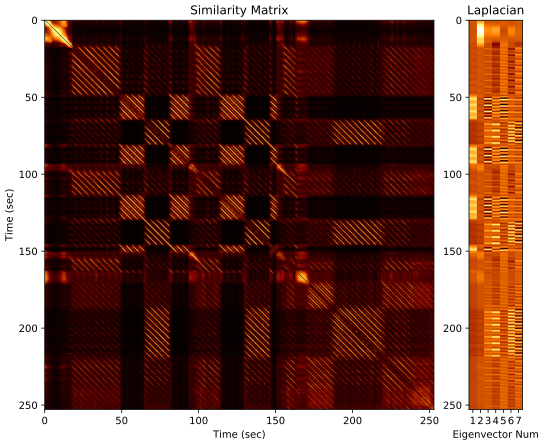
\includegraphics[width=0.85\columnwidth]{SimilarityMatrix_Laplacian.pdf}
    \caption{Similarity matrix $W^F$ and Laplacian eigenvectors after applying similarity network fusion to stack-delayed Chroma and MFCC features for the song ``Smooth Criminal'' by Michael Jackson.  The SSM and eigenvectors are much cleaner than those with just raw chroma in Figure~\ref{fig:SSMChroma}.}
    \label{fig:SSMFused}
   \end{figure}

\begin{figure}
    \centering
    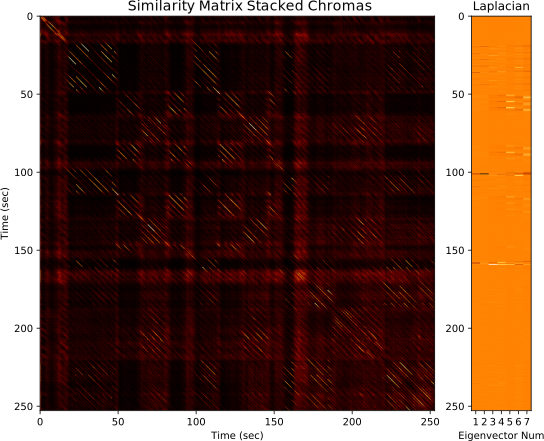
\includegraphics[width=0.85\columnwidth]{SimilarityMatrix_Chroma.pdf}
    \caption{Similarity matrix $W^C$ using the cosine distance on stack-delayed Chroma features, along with the corresponding weighted Laplacian eigenvectors.  While the stacked delay embedding helps diagonals to appear which indicate repeated structure, it is not as clean as the fused SSM in Figure~\ref{fig:SSMChroma}.}
    \label{fig:SSMChroma}
\end{figure}
   



\section{Visualizing Time-Ordered Similarity}

\begin{figure}
    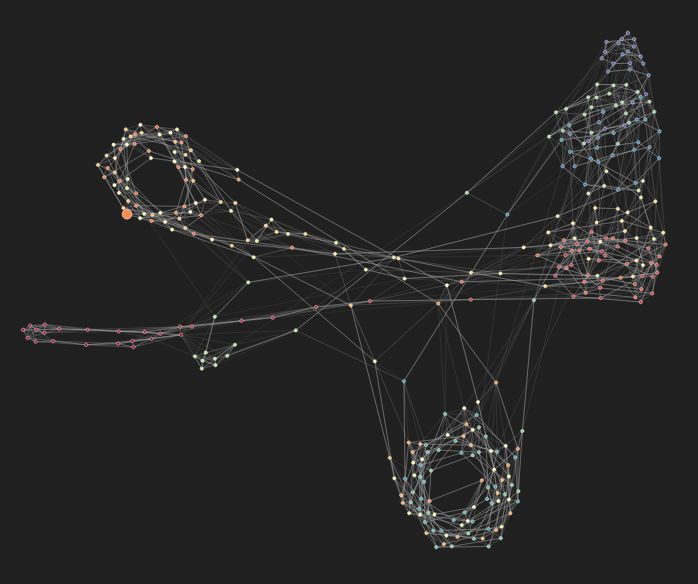
\includegraphics[width=\columnwidth]{ForceGraph.pdf}
    \caption{A dynamic weighted spring layout based on the weights in Figure~\ref{fig:SSMFused}, which is rendered with the help of d3.js \cite{bostock2012d3}.}
    \label{fig:ForceGraph}
\end{figure}
   
   
   
\begin{figure}
    \centering
    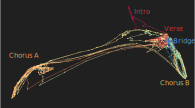
\includegraphics[width=0.8\columnwidth]{DiffusionMaps.pdf}
    \caption{3D Diffusion maps rendered by WebGL, synchronized to the music.}
    \label{fig:DiffusionMaps}
\end{figure}

The first facet of our GUI simply allows the user to view audio synchronized with the SSM, but enables a powerful way to visualize and jump between repeated elements in the song\footnote{This is similar to the cross-similarity GUI viewer we created for cover songs \cite{tralie2017cover}.}.  The second visualization performs a spring layout of the weighted graph induced from $W^F$, with the help of d3.js \cite{bostock2012d3}, as shown in Figure~\ref{fig:ForceGraph}.  Since we have applied a similarity kernel, the spring constant is proportional to how similar windows are; the simulation encourages more similar windows to be closer together.  Note that the simulation is dynamic; nodes in the graph can be moved around, and the simulation will settle in a local min of energy. Finally, we present a GUI for showing music synchronized to 3D diffusion maps \cite{coifman2006diffusion}.  This is the most similar GUI to our previous ``Loop Ditty'' GUI\cite{tralie2017Dissertation}, though it works purely on similarity information and not on coordinates in feature space, so it is much more general.


In future work, we would like to explore all of these structures for pruning in large scale audio cover song identification, similar to the aligned hierarchies work \cite{kinnaird2016aligned} on symbolic cover song identification.


% For bibtex users:
\small
\bibliography{main}


\end{document}
